% latex table generated in R 3.6.3 by xtable 1.8-4 package
% Thu Jan 18 11:48:41 2024
\begin{table}[ht]
\centering
\begin{tabular}{rlrrr}
  \hline
 & OTU & MeanRA & MedianRA & SE \\ 
  \hline
529 & Brucella anthrop & 0.00005521 & 0.00004333 & 0.00001307 \\ 
  1076596 & Acetobacter persic & 0.00003822 & 0.00003942 & 0.00000201 \\ 
  1591409 & Pseudohalocynthiibacter aestuariiviven & 0.00006874 & 0.00006454 & 0.00000340 \\ 
  1705310 & Burkholderia sp. IDO & 0.00003881 & 0.00003858 & 0.00000155 \\ 
  2498848 & Pseudomonas sp. MPC & 0.00006114 & 0.00005150 & 0.00000601 \\ 
  253237 & Pseudomonas sp. phDV & 0.00003056 & 0.00001690 & 0.00000720 \\ 
  200450 & Pseudomonas triviali & 0.00007569 & 0.00007215 & 0.00000608 \\ 
  86185 & Pseudomonas lundensi & 0.00005308 & 0.00004848 & 0.00000467 \\ 
  1853130 & Pseudomonas silesiensi & 0.00004971 & 0.00004564 & 0.00000416 \\ 
  46677 & Pseudomonas agaric & 0.00005263 & 0.00004495 & 0.00000606 \\ 
  83655 & Leclercia adecarboxylat & 0.00004420 & 0.00004495 & 0.00000202 \\ 
  565 & Atlantibacter hermanni & 0.00002558 & 0.00002652 & 0.00000135 \\ 
  2769486 & Marinobacter sp. LPB031 & 0.00005386 & 0.00005341 & 0.00000242 \\ 
  550540 & Ferrimonas balearica & 0.00006981 & 0.00006809 & 0.00000247 \\ 
  1704499 & Methylovulum psychrotoleran & 0.00003183 & 0.00003102 & 0.00000135 \\ 
  2738883 & Candidatus Reidiella endopervernicos & 0.00005277 & 0.00004928 & 0.00000355 \\ 
  43771 & Corynebacterium urealyticu & 0.00006230 & 0.00006477 & 0.00000286 \\ 
  146827 & Corynebacterium simulan & 0.00003860 & 0.00003685 & 0.00000419 \\ 
  544580 & Actinomyces ori & 0.00004523 & 0.00004344 & 0.00000242 \\ 
  181487 & Schaalia cardiffensi & 0.00003705 & 0.00003564 & 0.00000251 \\ 
  1684 & Bifidobacterium asteroide & 0.00003416 & 0.00003500 & 0.00000306 \\ 
  1944646 & Phoenicibacter congonensi & 0.00001412 & 0.00001540 & 0.00000252 \\ 
  79263 & Paenibacillus chitinolyticu & 0.00006362 & 0.00006648 & 0.00000308 \\ 
  375489 & Paenibacillus cellulosilyticu & 0.00005710 & 0.00005702 & 0.00000337 \\ 
  365617 & Paenibacillus sabina & 0.00004806 & 0.00004928 & 0.00000223 \\ 
  2610894 & Flintibacter & 0.00004676 & 0.00004702 & 0.00000305 \\ 
  42837 &   & 0.00006710 & 0.00006762 & 0.00000274 \\ 
  907 & Megasphaera elsdeni & 0.00004887 & 0.00004830 & 0.00000224 \\ 
  552811 &   & 0.00006157 & 0.00006108 & 0.00000396 \\ 
  2528007 & Polystyrenella long & 0.00006108 & 0.00005642 & 0.00000461 \\ 
  353800 & Halostagnicola larseni & 0.00005693 & 0.00005240 & 0.00000319 \\ 
  1229908 & Candidatus Nitrosopumilus koreensis & 0.00000604 & 0.00000443 & 0.00000156 \\ 
   \hline
\end{tabular}
\caption{Keystone OTUs of } 
\end{table}
\begin{figure}
\centering
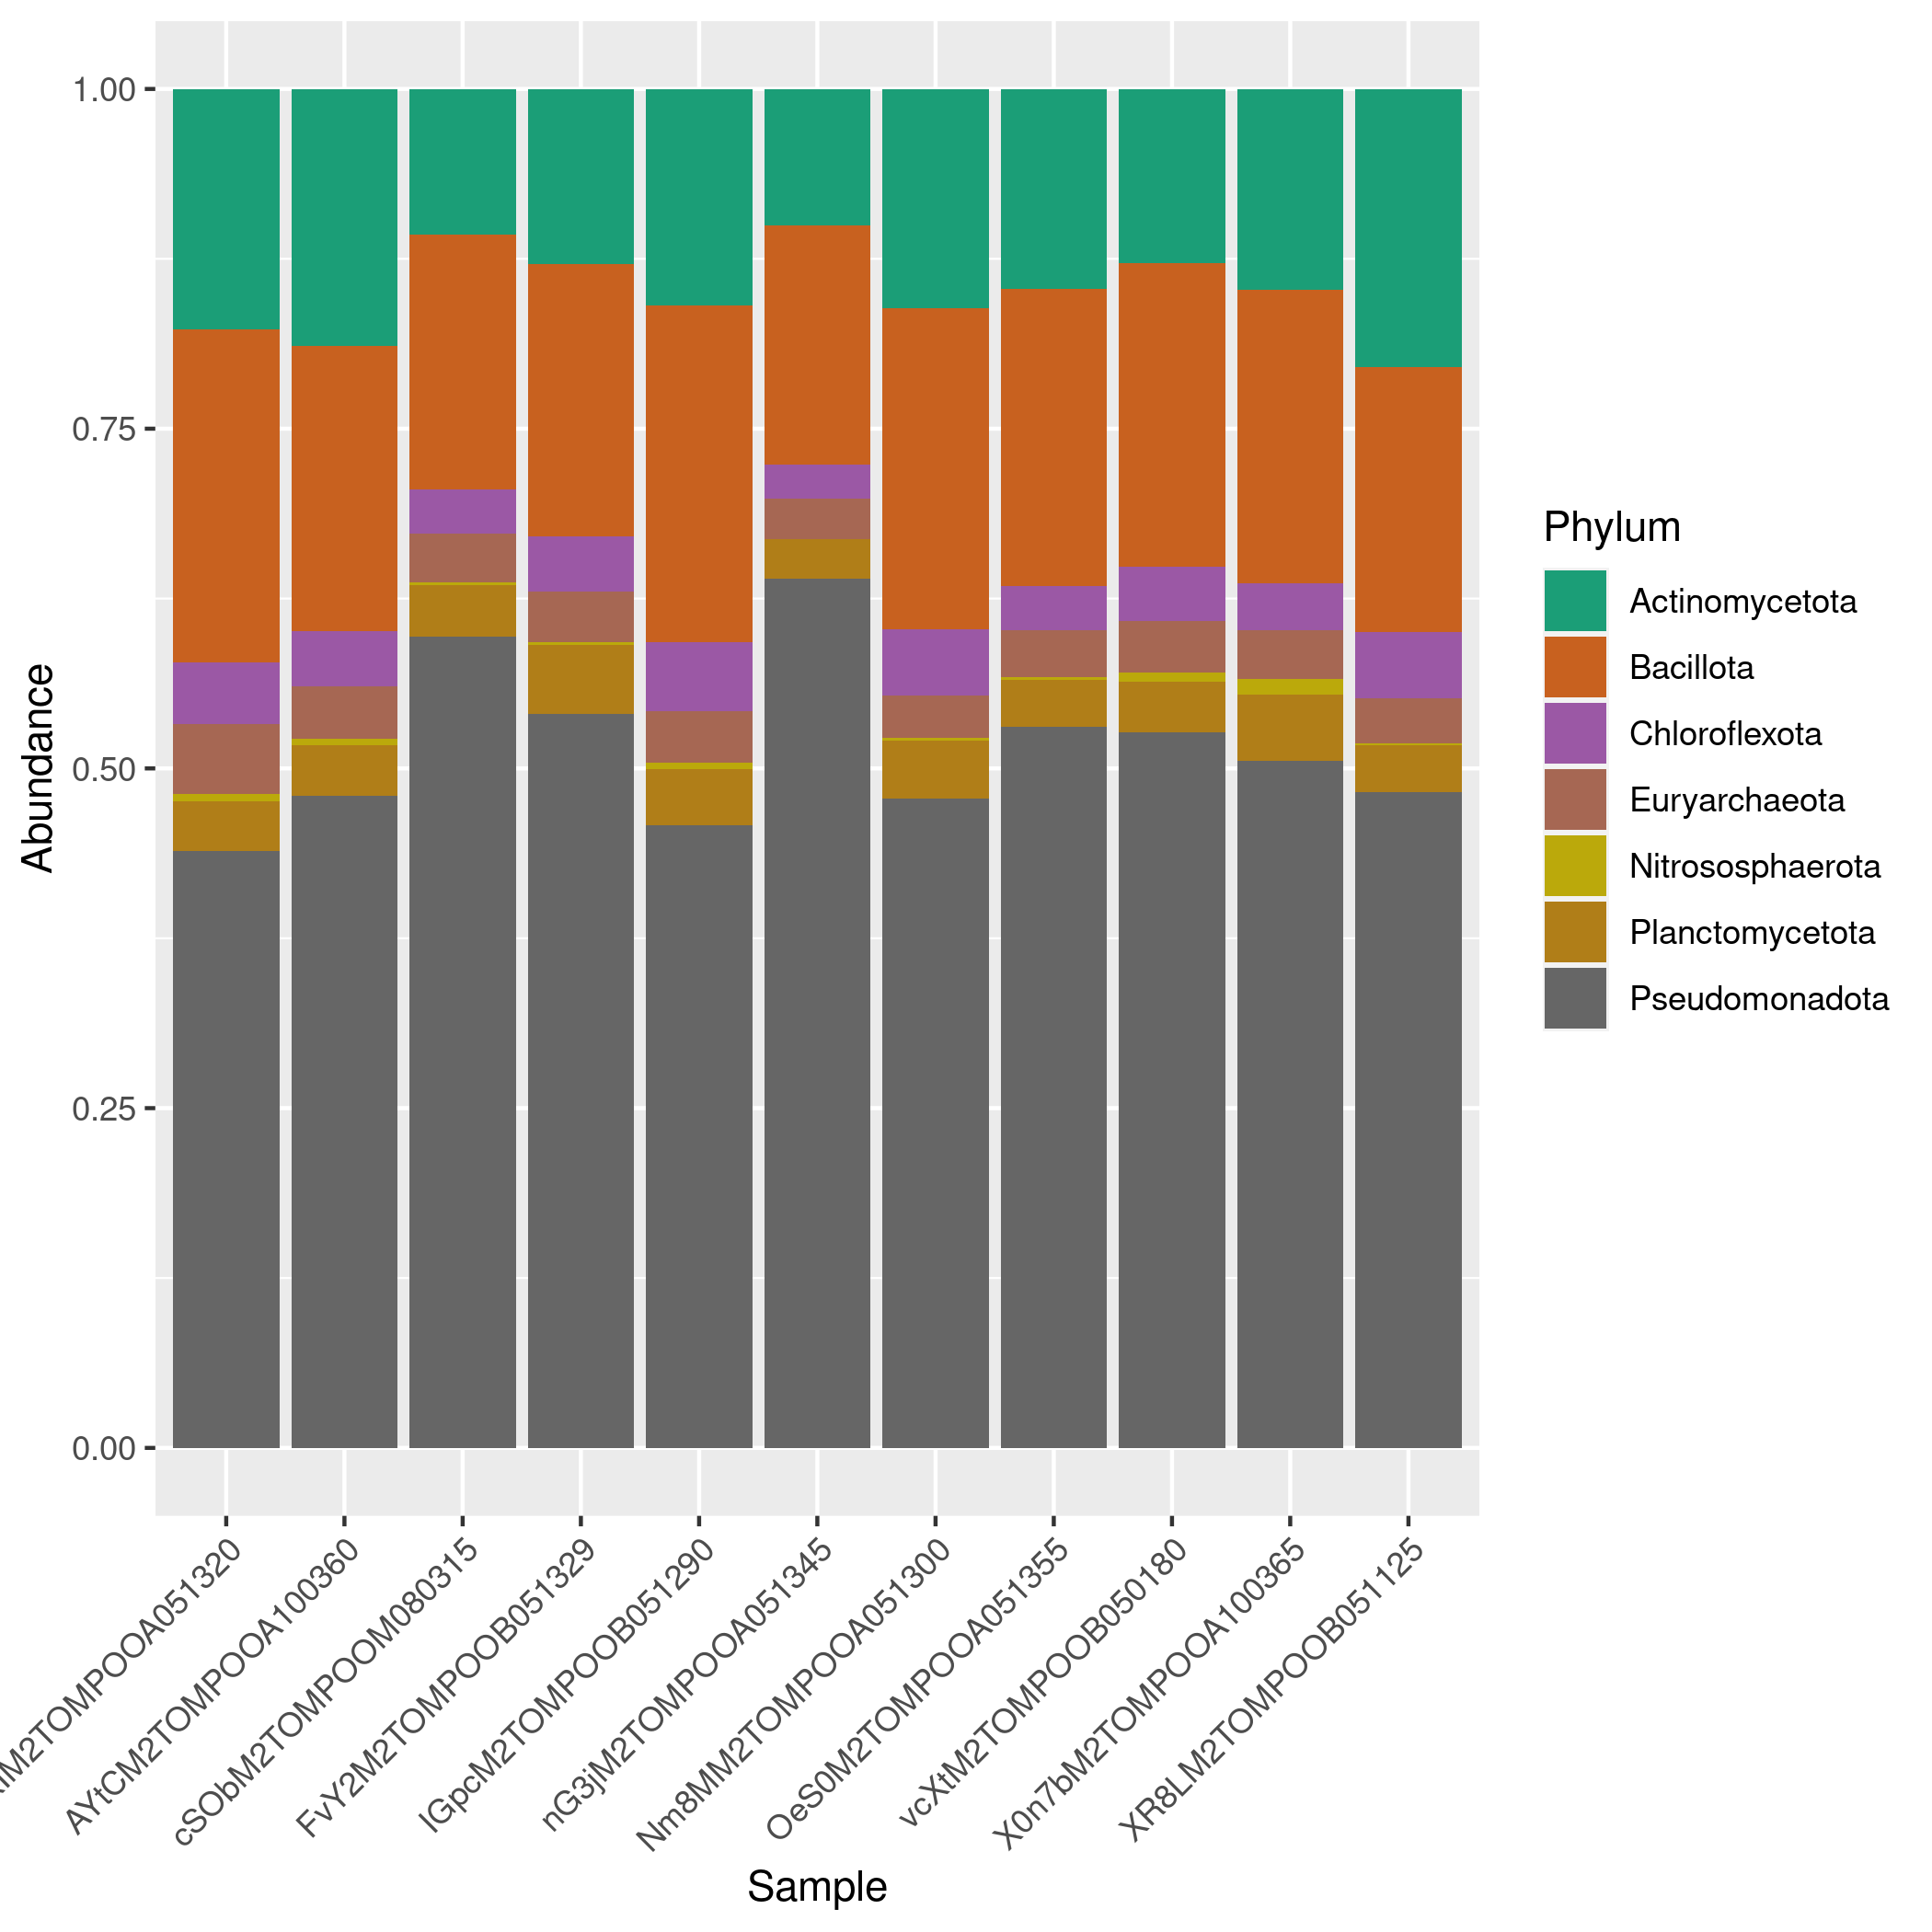
\includegraphics[scale = 0.8]{tomate_aleatorio1_7.csv_relative_abundance_Phylum.png}
\caption{Relative abundance by phyla of keystone OTUs }
\label{fig:tomate_aleatorio1_7.csv_phyla}
\end{figure}
\begin{figure}
\centering
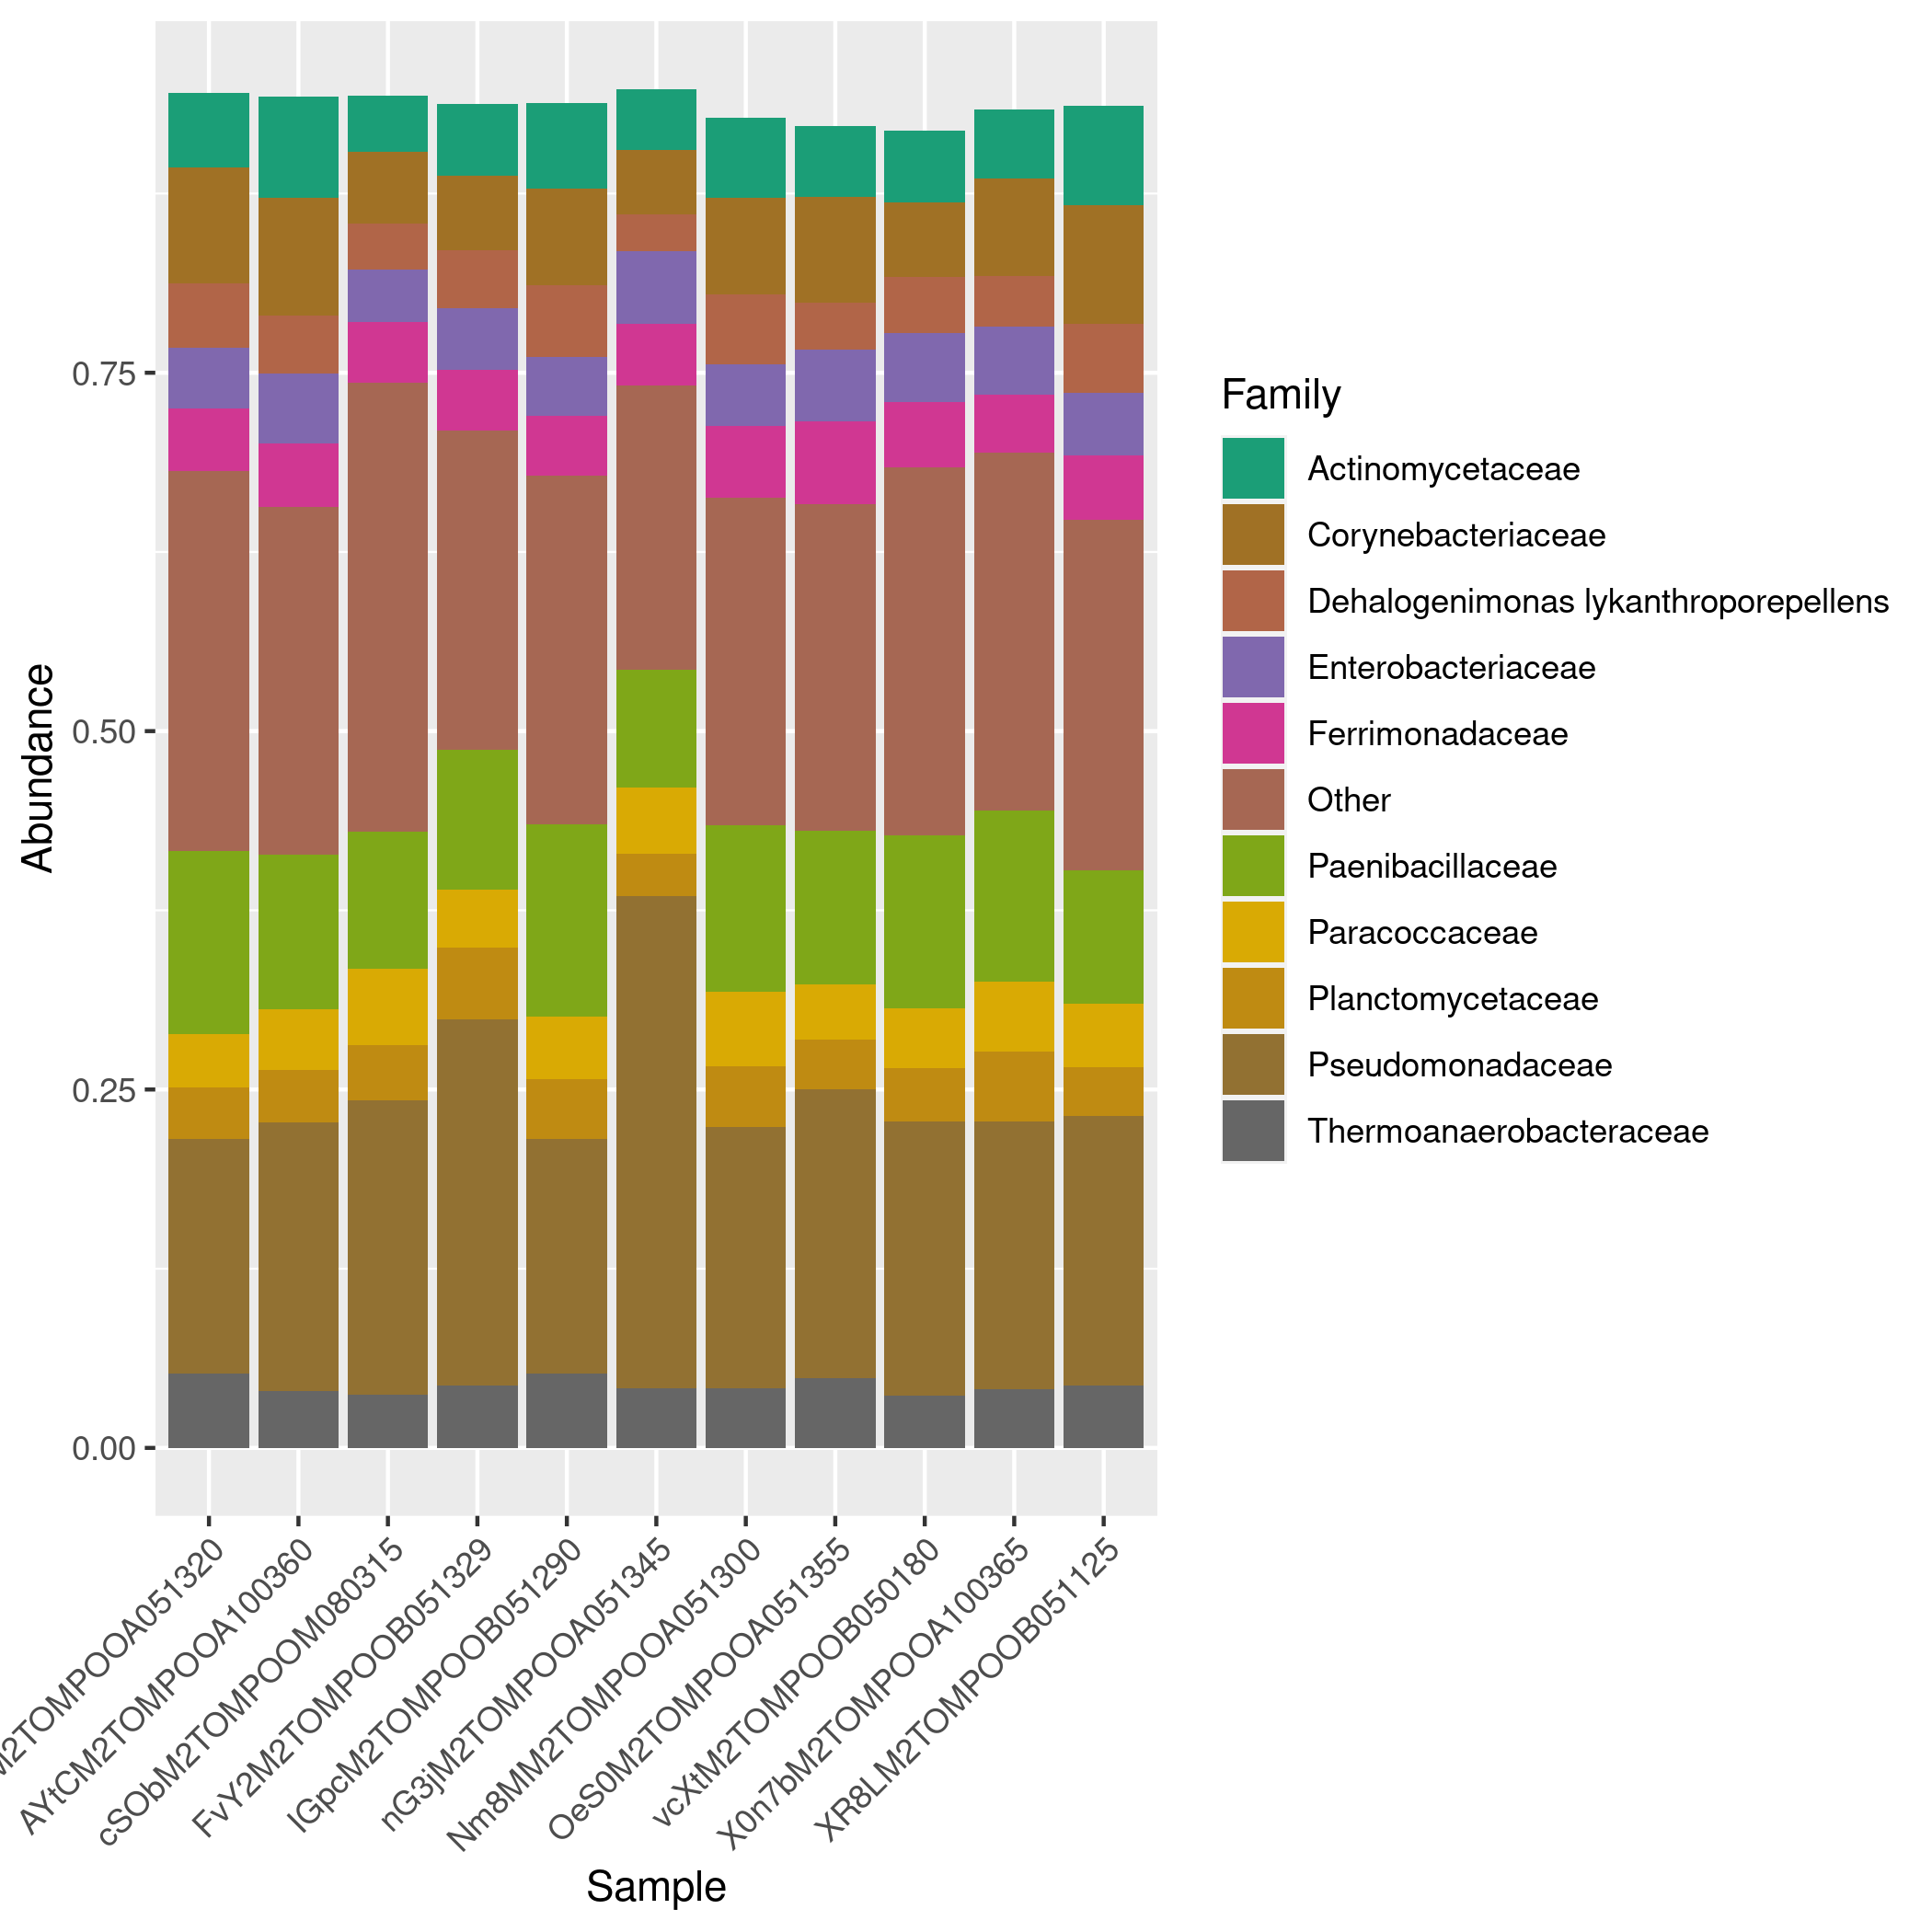
\includegraphics[scale = 0.8]{tomate_aleatorio1_7.csv_relative_abundance_Family.png}
\caption{Relative abundance by families of keystone OTUs }
\label{fig:tomate_aleatorio1_7.csv_family}
\end{figure}
\begin{figure}
\centering
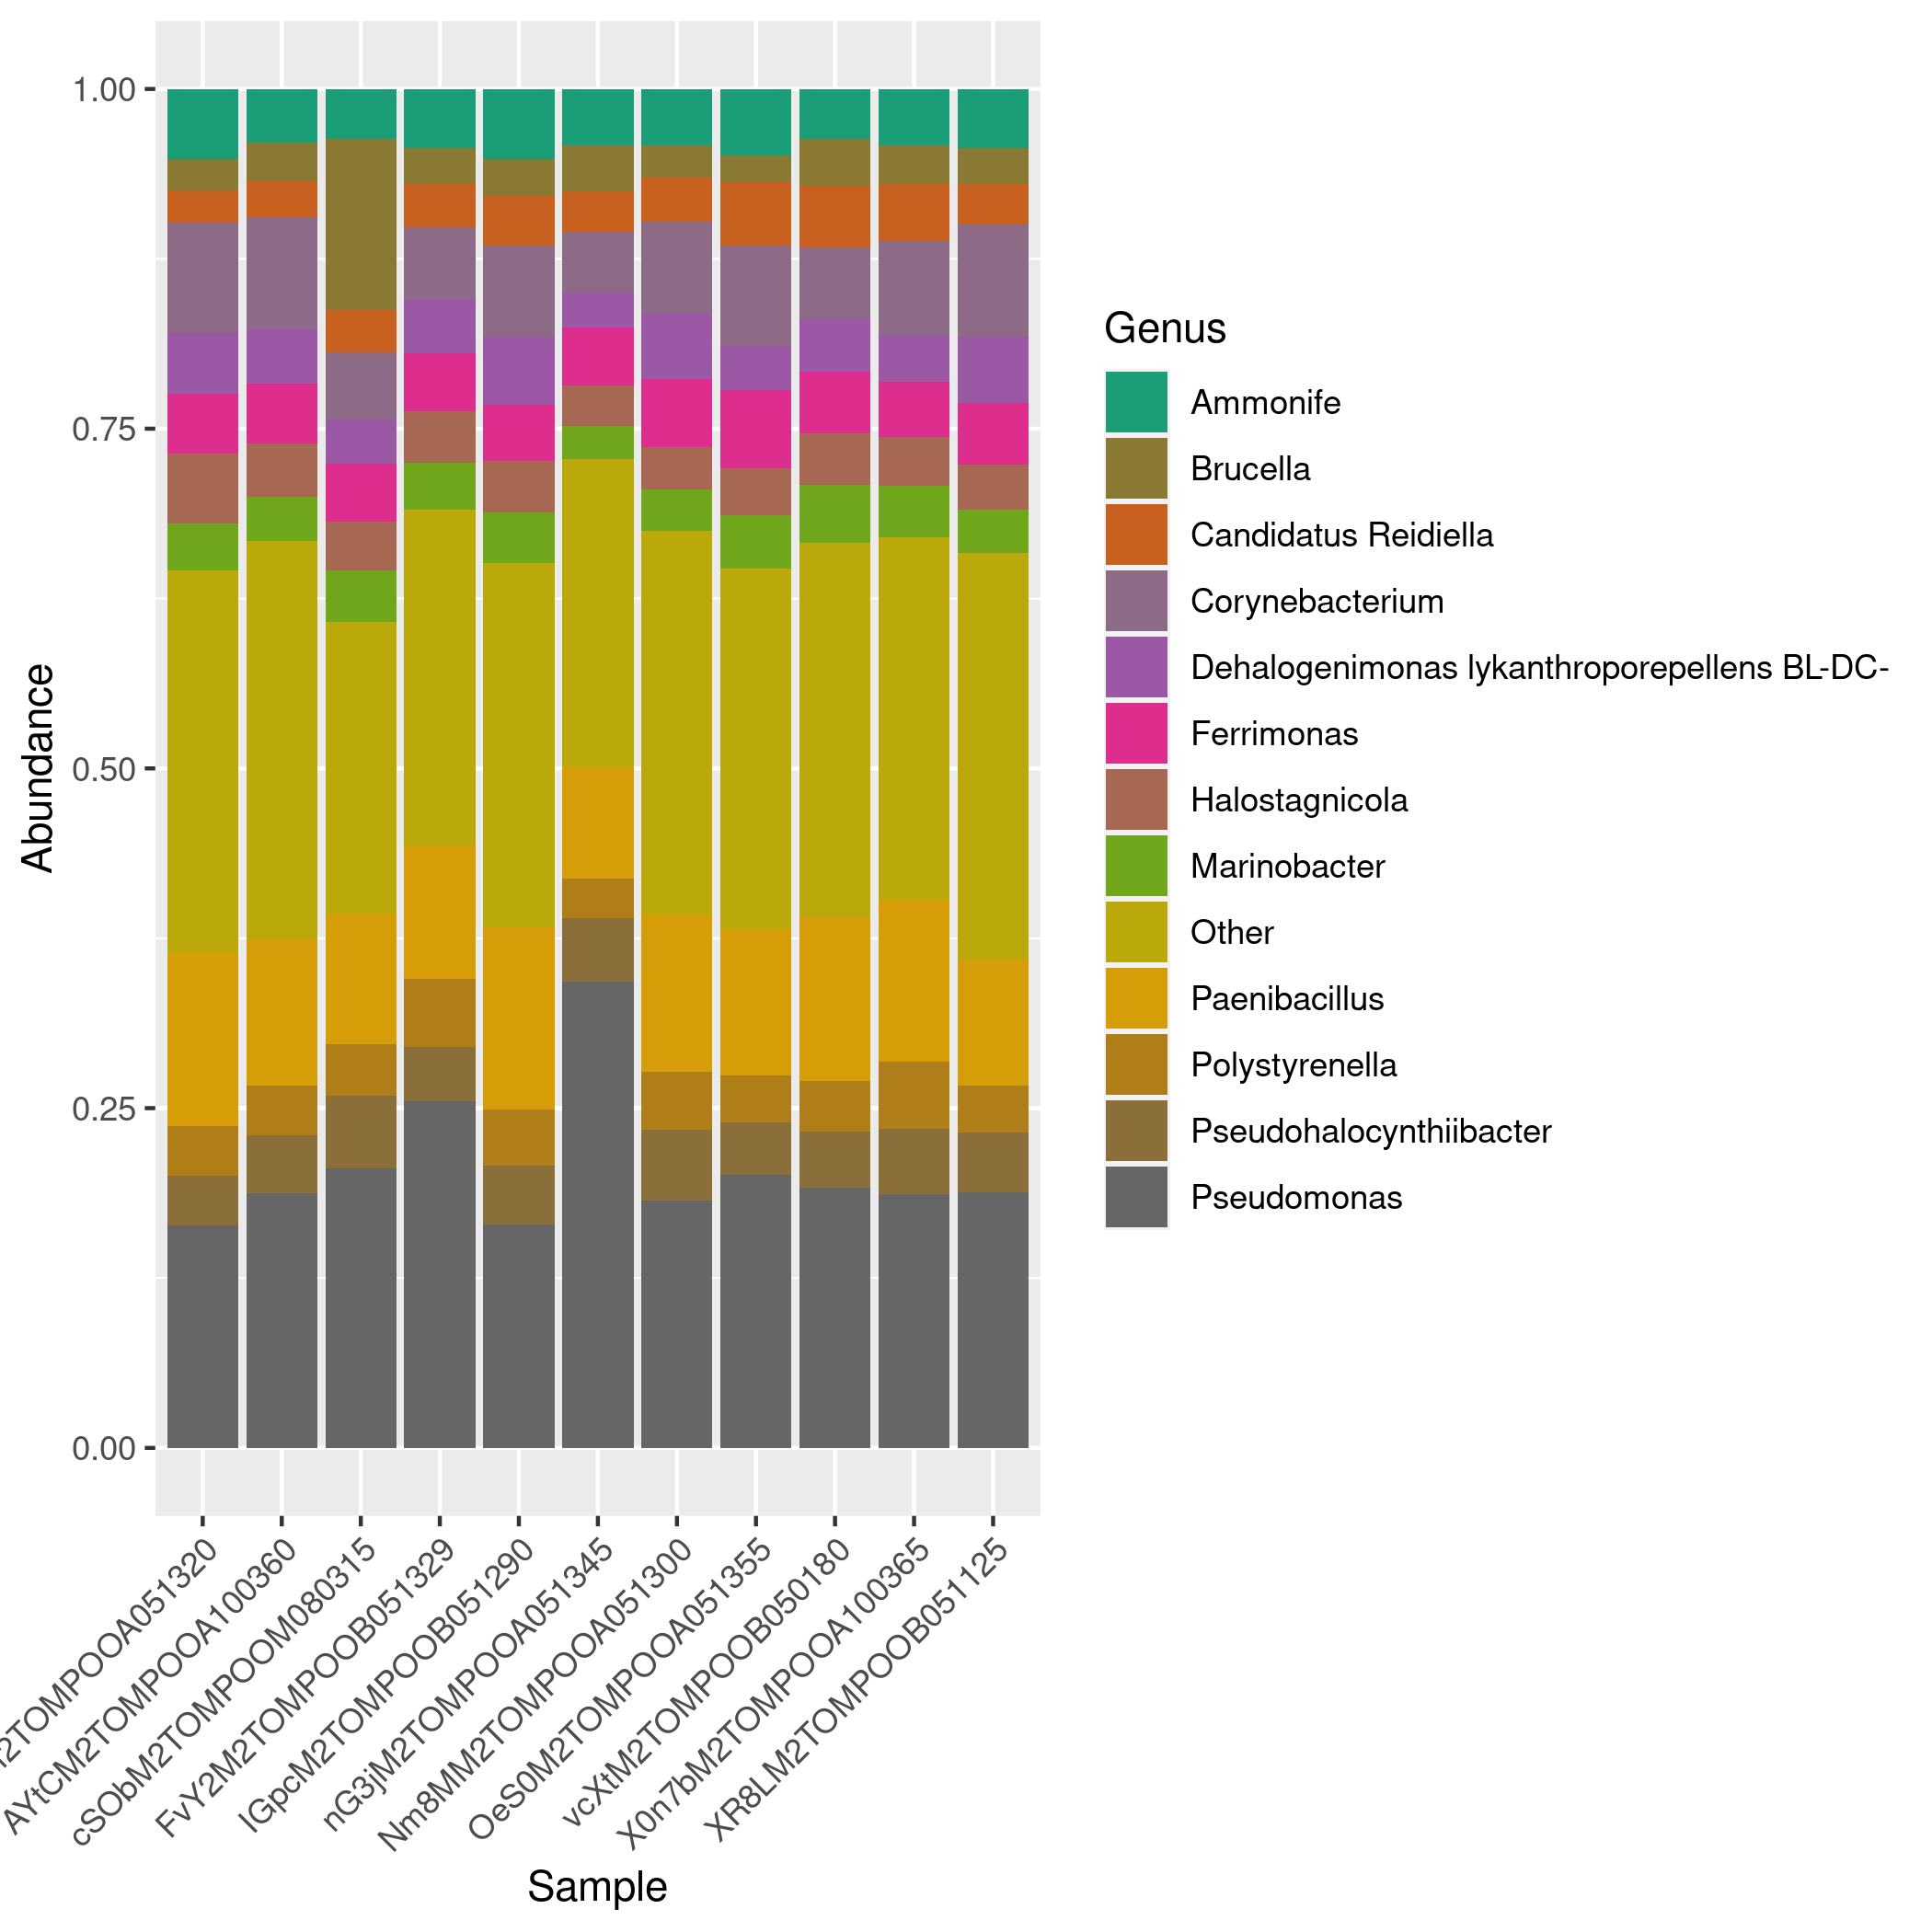
\includegraphics[scale = 0.8]{tomate_aleatorio1_7.csv_relative_abundance_Genus.png}
\caption{Relative abundance by genera of keystone OTUs }
\label{fig:tomate_aleatorio1_7.csv_genus}
\end{figure}
\begin{figure}
   \centering
   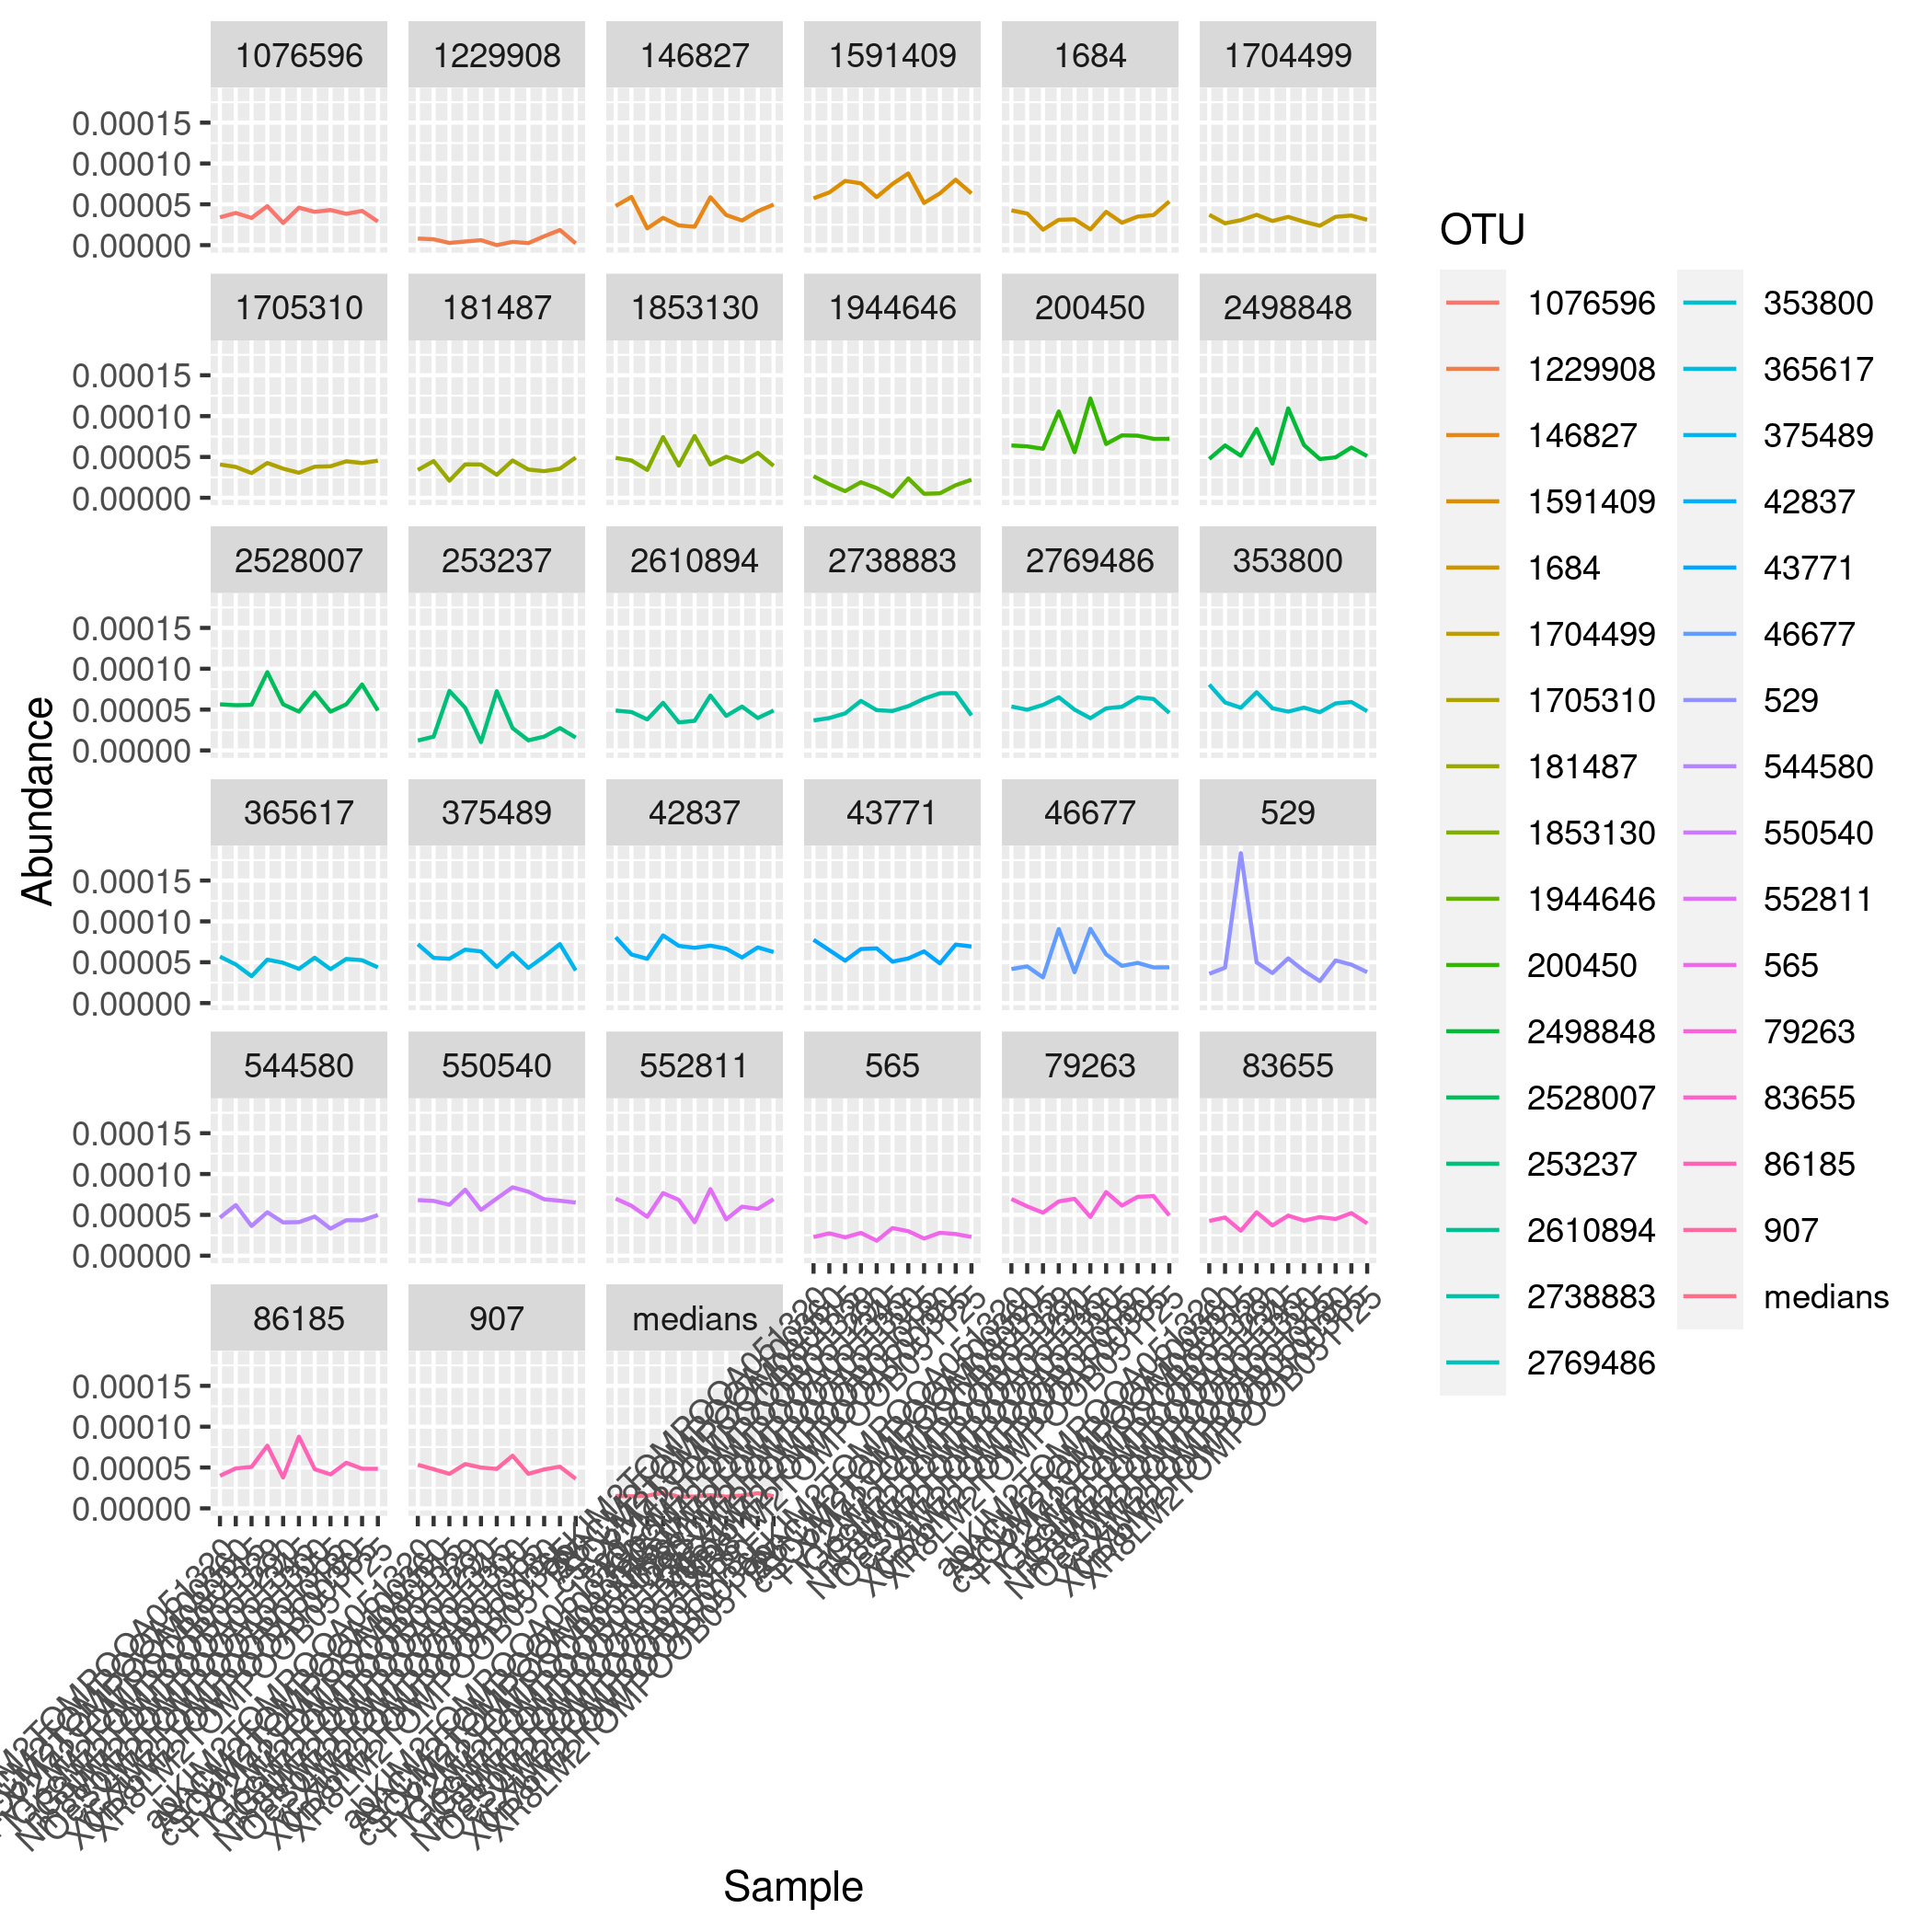
\includegraphics[scale = 0.8]{abundance_tomate_aleatorio1_7.csv_key_otus_medians.png}
   \caption{Plots representing relative abundance of each keystone OTU and one representing the median relative abundance  across samples of rhizosphere of tomate_aleatorio1_7.csv. Most keystone OTUs have relative abundance bigger than the median across all samples.  }
   \label{key_otus_vs_medians_tomate_aleatorio1_7.csv}
\end{figure}
\begin{figure}
 \centering
 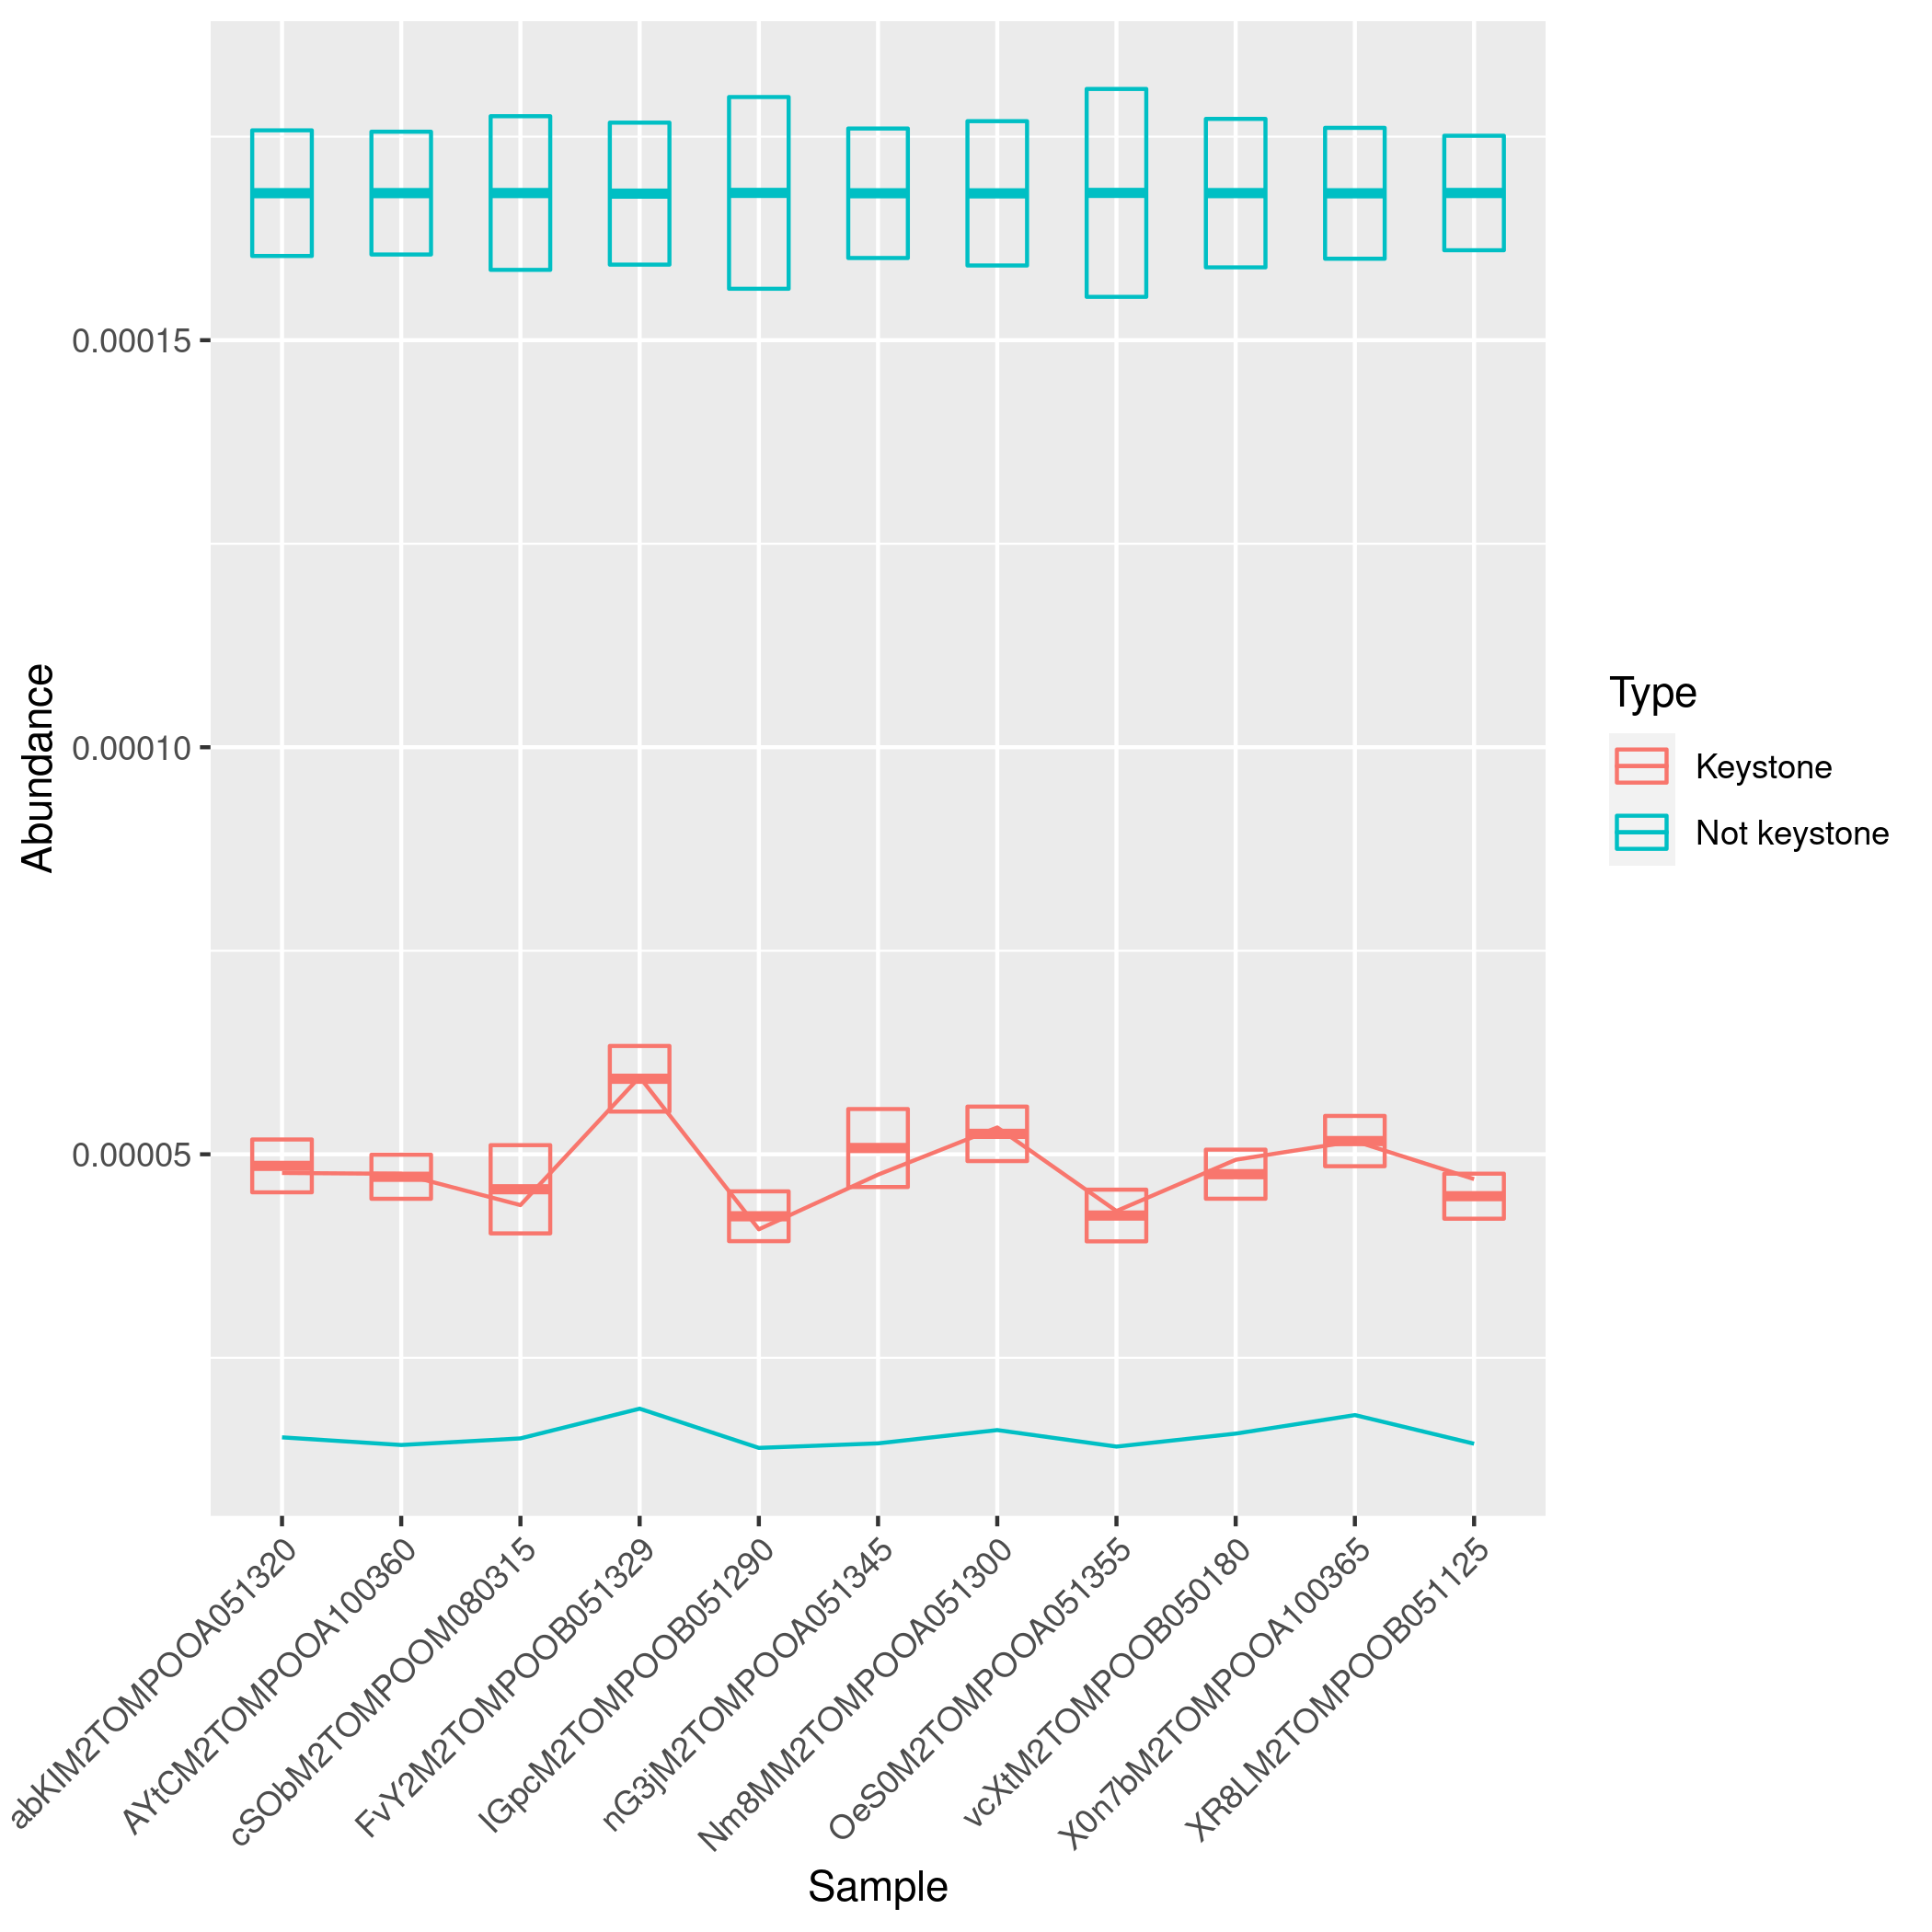
\includegraphics[scale = 0.75]{mean_median_key_vs_not_key_tomate_aleatorio1_7.csv.png}
\caption{Boxes represent mean and standard error in the distribution of corresponding samples. Lines represent the corresponding medians. In these samples of rhizosphere oftomate_aleatorio1_7.csv}
\label{mean_median_tomate_aleatorio1_7.csv}
\end{figure}
\begin{figure}
   \centering
   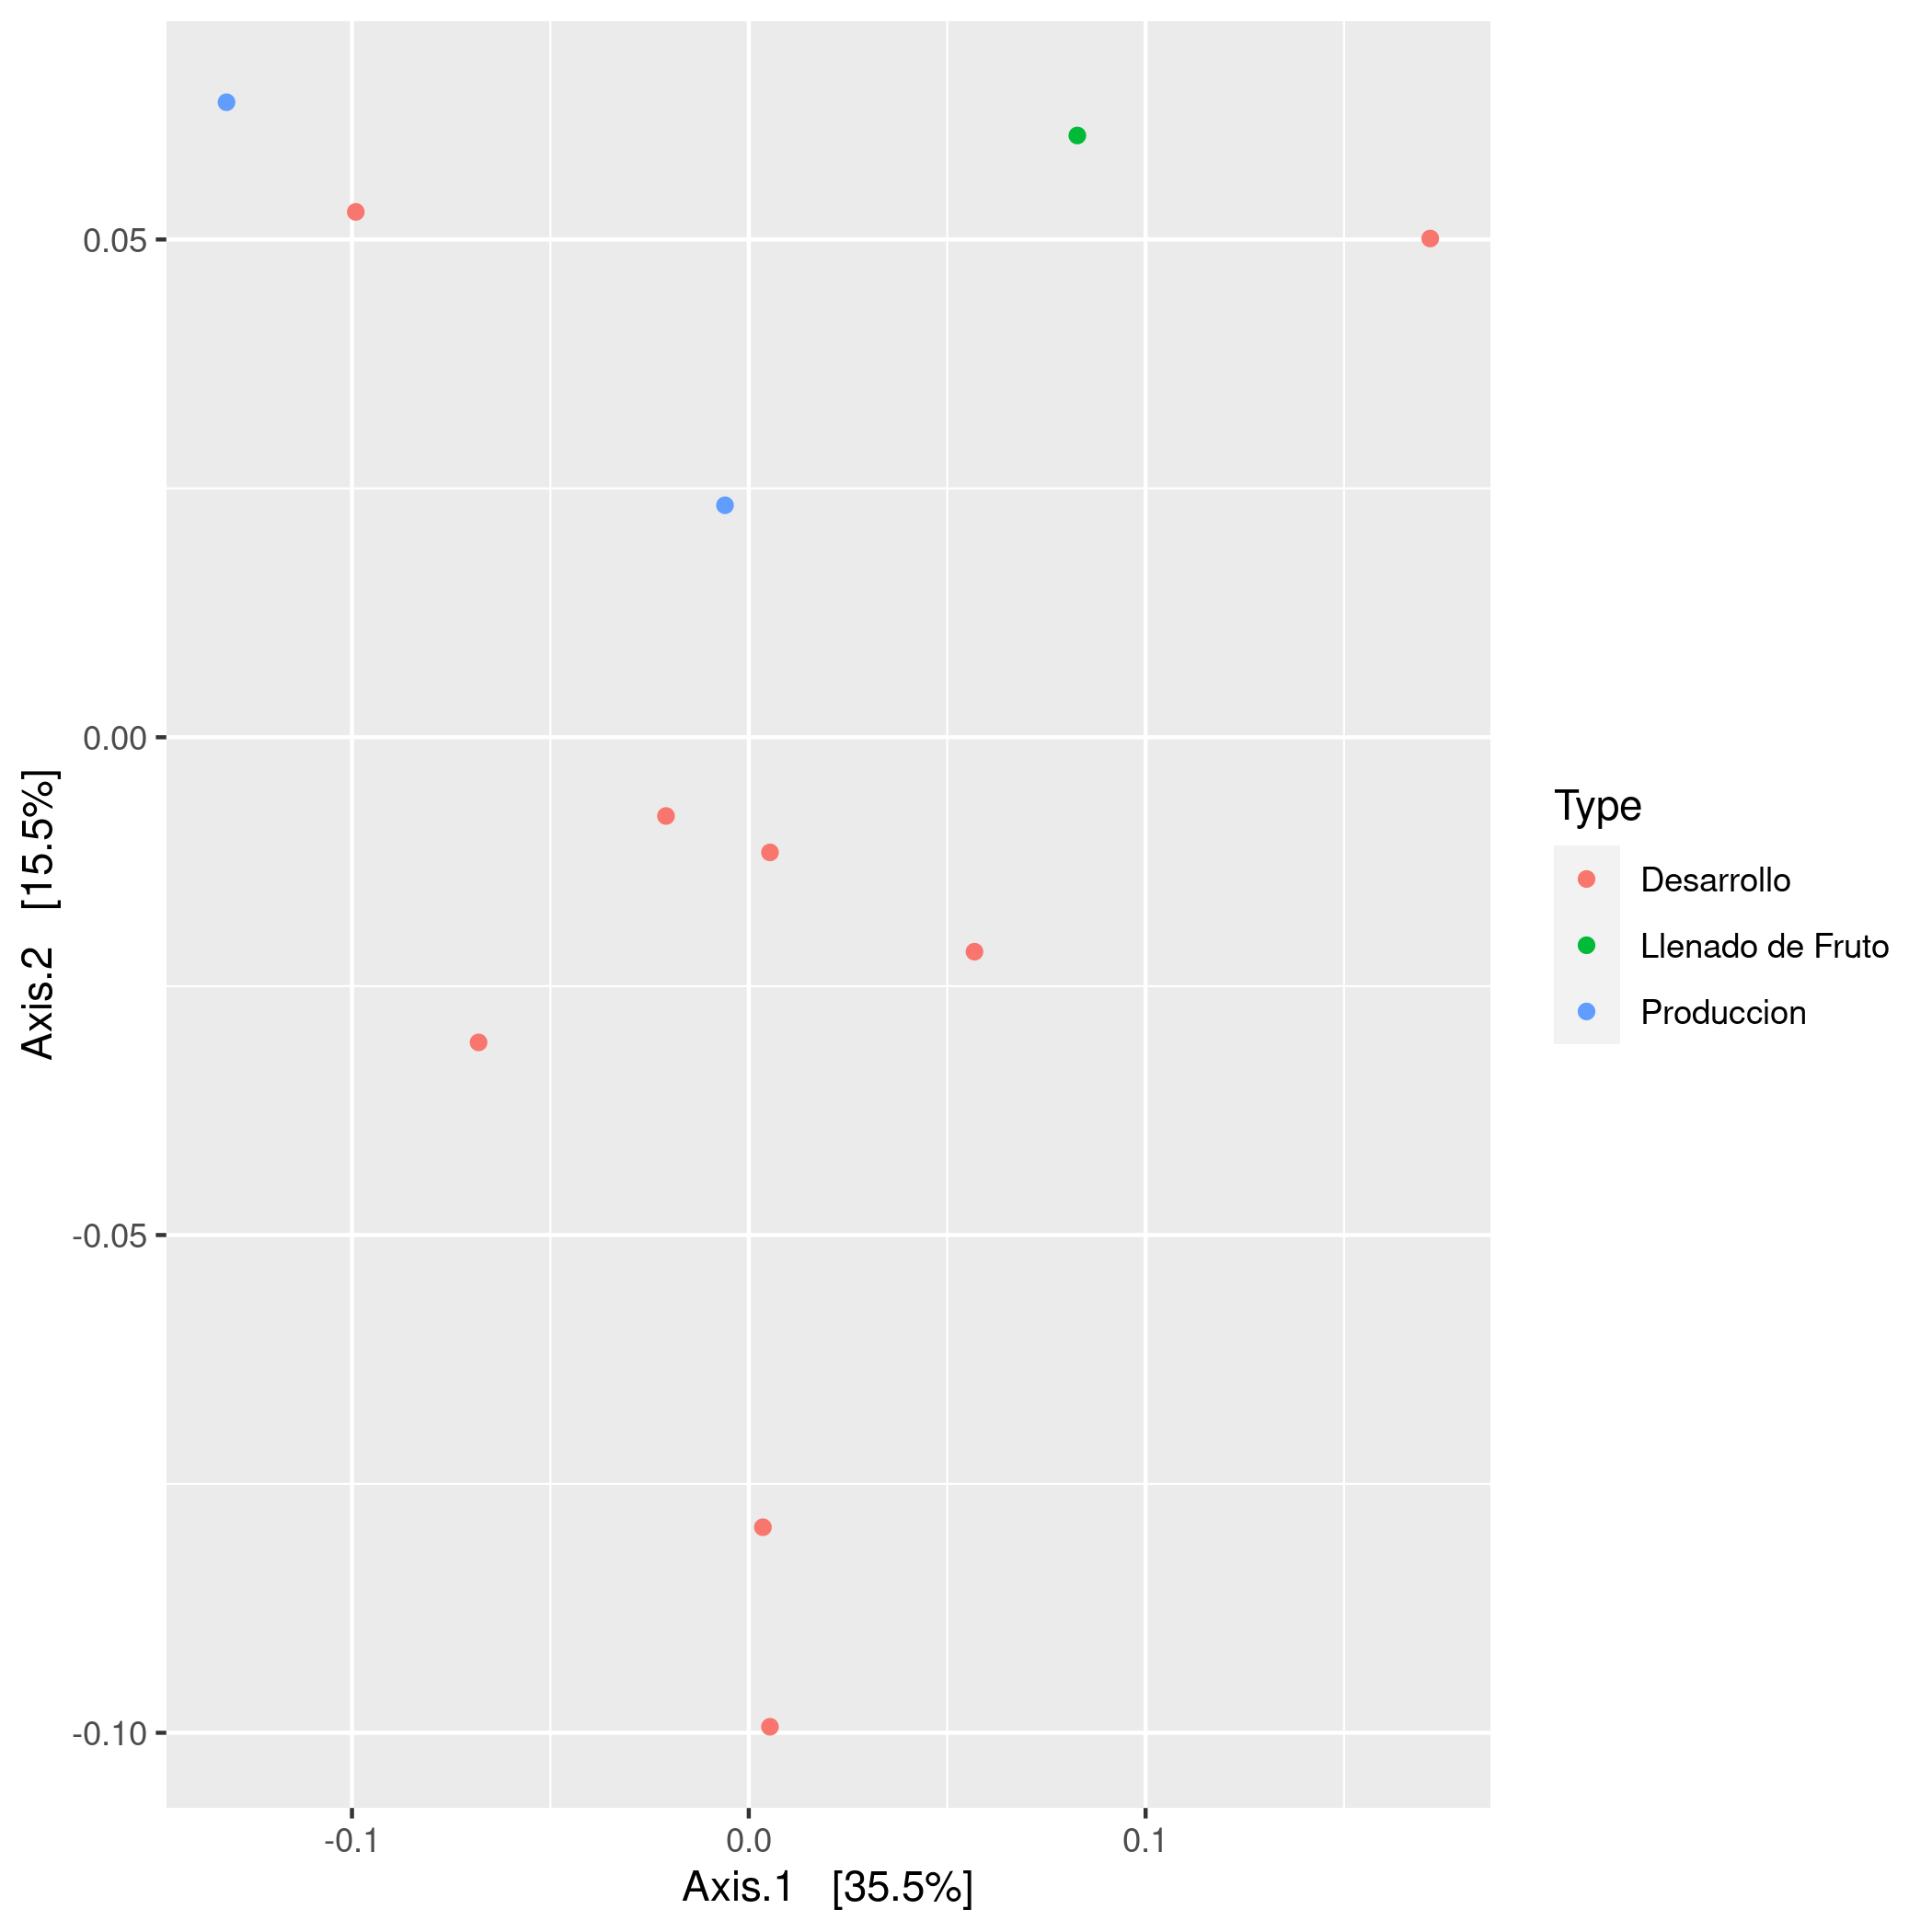
\includegraphics[scale = 0.7]{pcoa_muestras_tomate_aleatorio1_7.csv.png}
 \caption{PCoA analysis with Bray-Curtis distance of rhizosphere samples of tomate_aleatorio1_7.csv.}
 \label{fig:tomate_aleatorio1_7.csv_pcoa}
\end{figure}
\begin{figure}
  \centering
  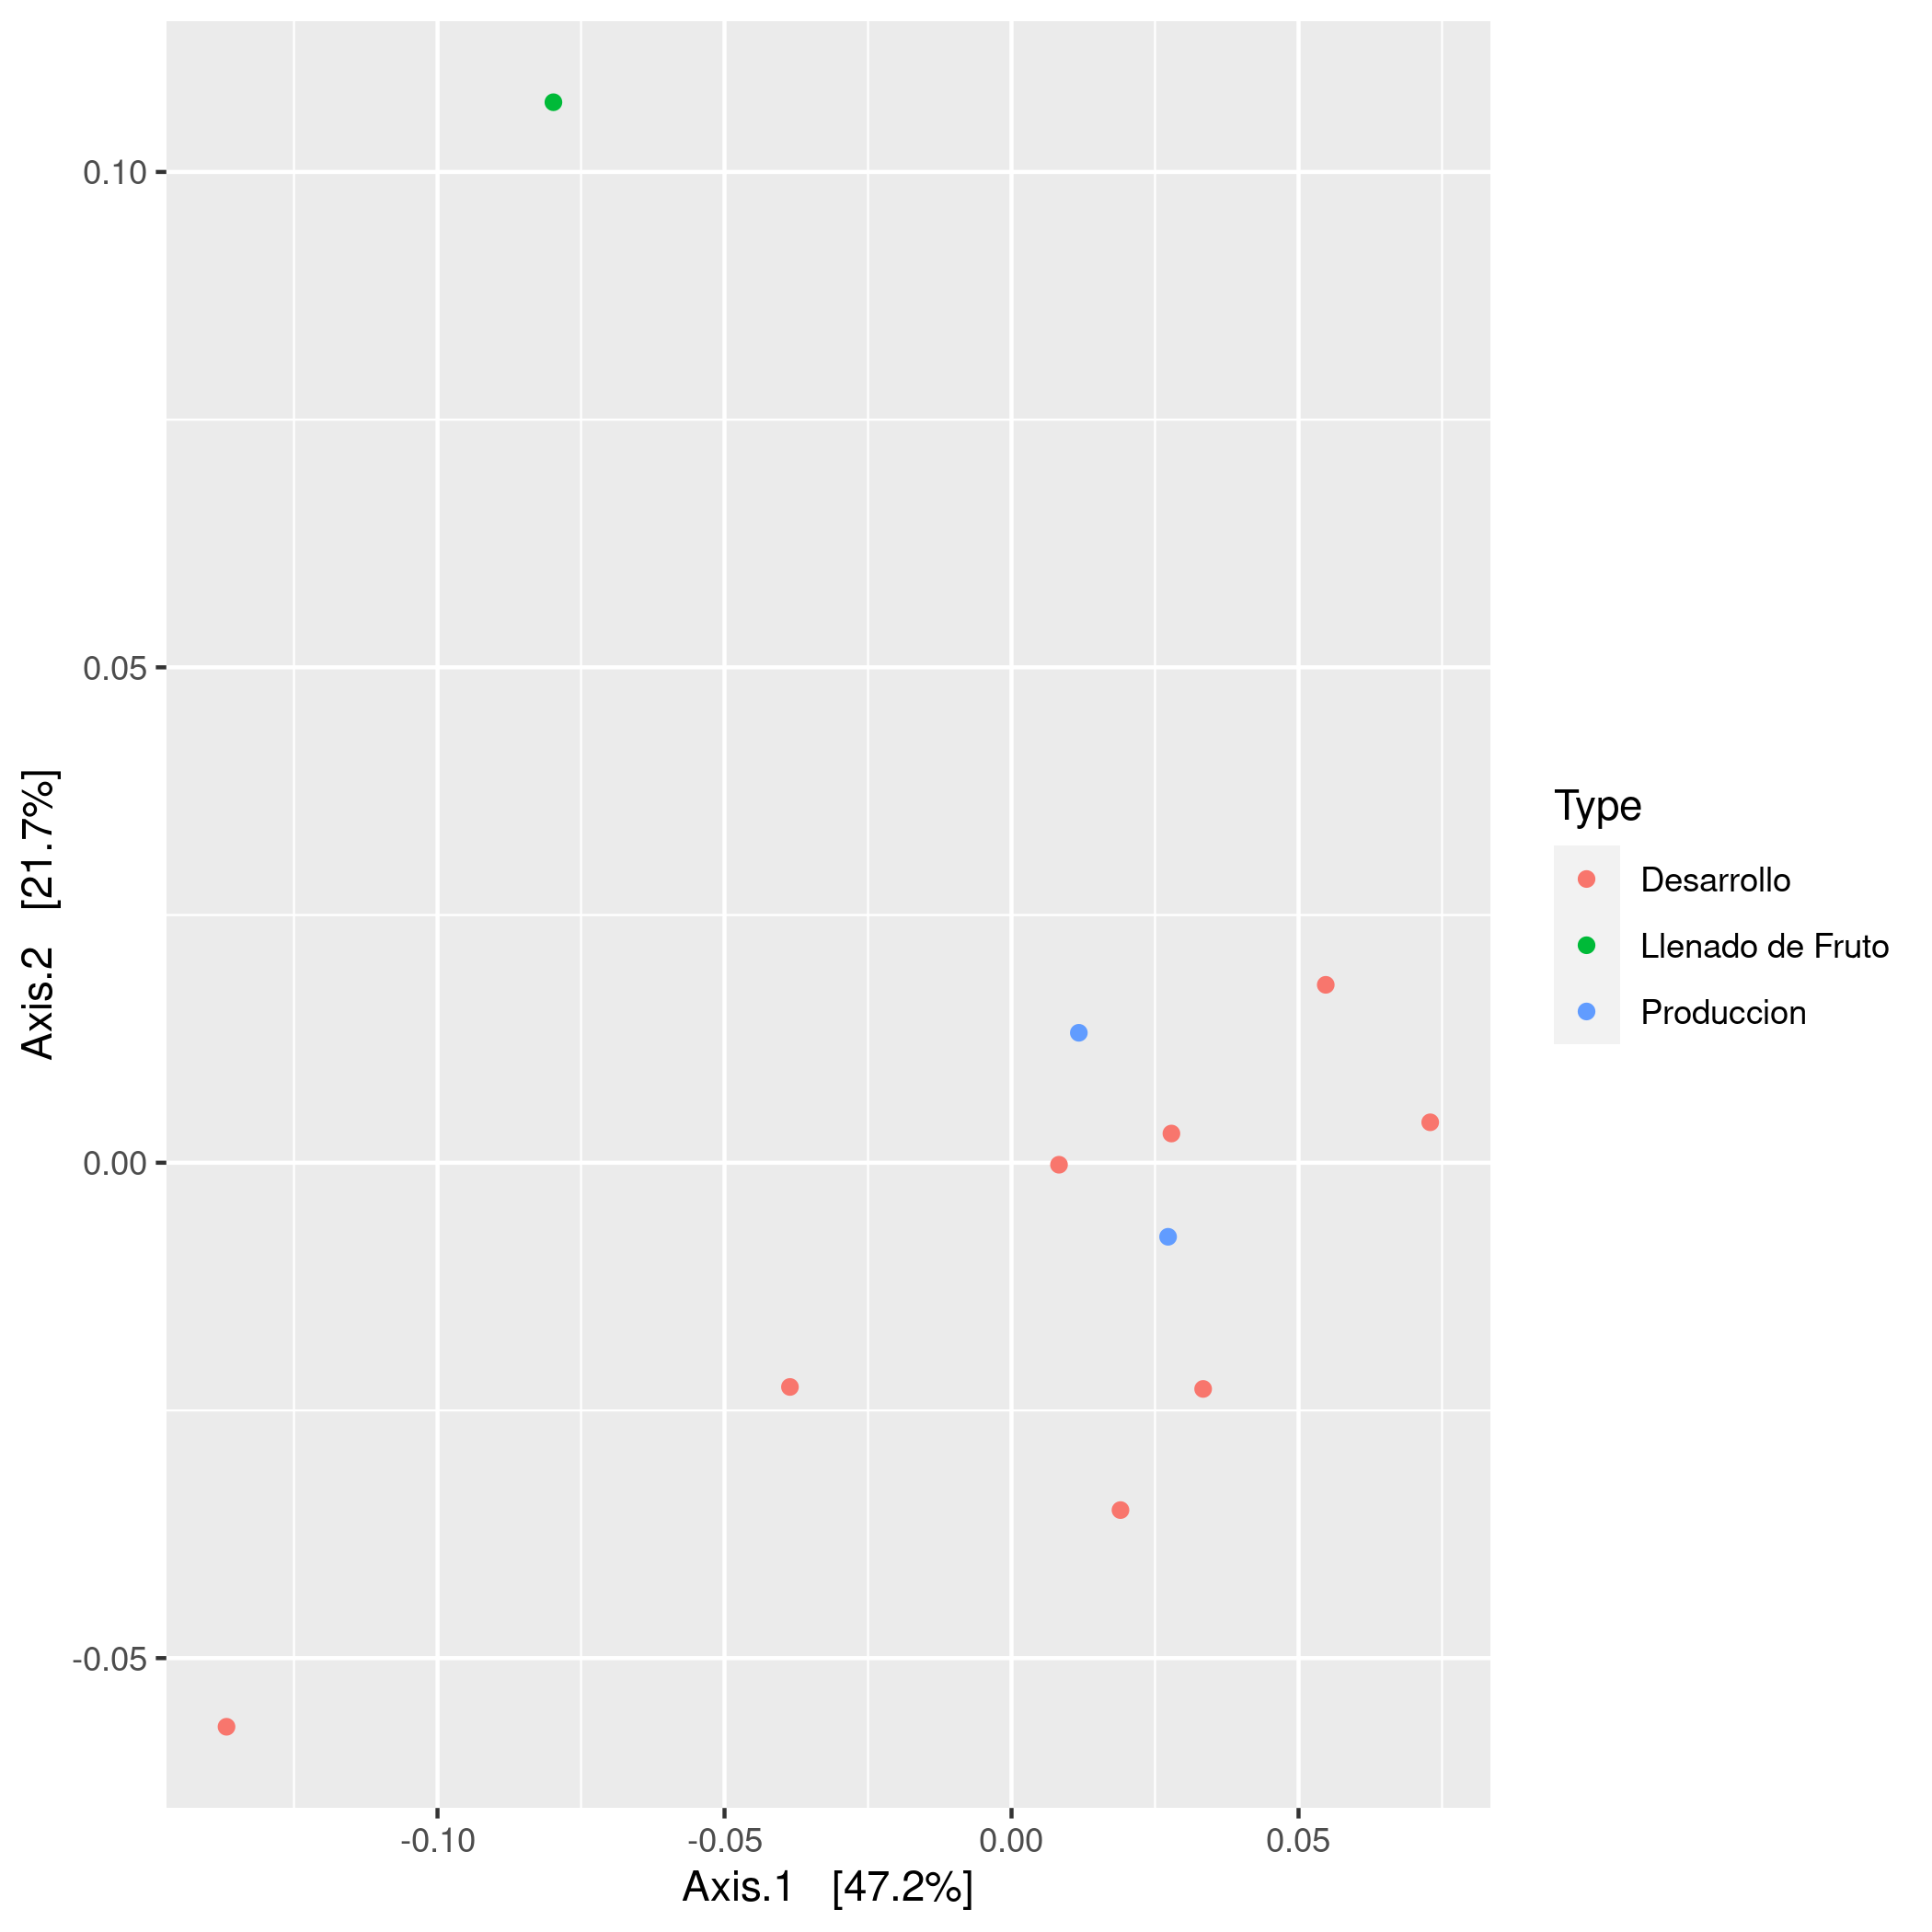
\includegraphics[scale = 0.7]{pcoa_key_otus_tomate_aleatorio1_7.csv.png}
  \caption{PCoA analysis with Bray-Curtis distance of rhizosphere samples of tomate_aleatorio1_7.csv, restricted to keystone OTUs.}
  \label{fig:tomate_aleatorio1_7.csv_pcoa_key_otus}
\end{figure}
